\documentclass{beamer}
\usetheme{Malmoe}
\usepackage{minted}
\usepackage{hyperref}
\usepackage{listings}


\title[Kivy]{Kivy: a sweet new app development framework}

\begin{document}


\begin{frame}[plain]
  \titlepage
\end{frame}


\begin{frame}{hey who let you in here}
my experience with mobile/desktop apps:

\pause
\begin{itemize}
  \item Kivy user since Saturday
  \pause
  \item ETS (TraitsUI, Chaco) for numpy/scipy-type apps
  \pause
  \item Occasionally fiddle with Qt and friends: PyQT4, pyside
  \pause
  \item I tried to do something with pygame once but got bored
\end{itemize}
\end{frame}


\begin{frame}{the skinny}
\begin{itemize}
  \item Fast
    \pause
    \begin{itemize}
    \item graphics system implemented OpenGL ES 2.0
    \pause
    \item important bits written in C/Cython
    \end{itemize}
  \pause
  \item Simple: beautiful API
  \pause
  \item Multitouchtouchtouch
  \pause
  \item Crossplatform: Linux, Windows, OSX, Android
  \pause
  , ...iOS?
  \pause
  \item License: LGPL3
\end{itemize}
\end{frame}


\begin{frame}{howsisworkthen?}

\begin{center}
  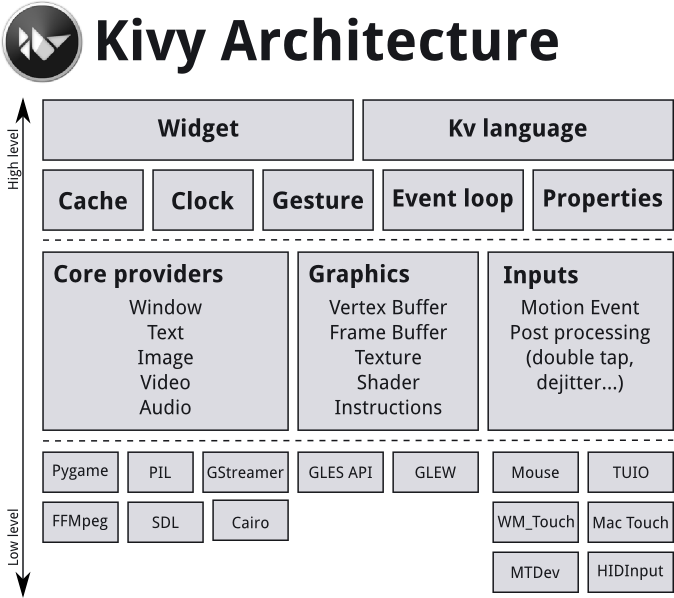
\includegraphics[height=.75\textheight]{architecture.png}
\end{center}

source: http://kivy.org/docs/guide/architecture.html

\end{frame}


\begin{frame}{widgets}
Widgets are...
\pause
\begin{itemize}
  \item anything you draw
  \pause
  \item anything you touch
  \pause
  \item anything you want to remember (data)
  \pause
  \item trees
    \begin{itemize}
    \pause
    \item there's always at least one root widget
    \pause
    \item parent.add\_widget(child) - attach a widget
    \pause
    \item parent.children - a list of widgets
    \pause
    \item parent.remove\_widget(child) - remove a widget
    \pause
    \item parent.clear\_widgets() - remove all widgets
    \end{itemize}
\end{itemize}
\end{frame}


\begin{frame}[fragile]{hello world}
  \inputminted{python}{hello_world.py}
\end{frame}


\begin{frame}{properties}
  Widgets can have properties. Properties are values you can bind callback functions to.
  \pause

  Examples:
    \begin{itemize}
    \item StringProperty
    \pause
    \item ListProperty
    \pause
    \item BooleanProperty
    \pause
    \item ObjectProperty
    \end{itemize}
\end{frame}


\begin{frame}[fragile]{property example}
  \inputminted{python}{property_example.py}
\end{frame}


% \begin{frame}{final note on properties}
%   You can also register and dispatch custom events if you need to get fancy.
% \end{frame}


\begin{frame}{clock}
There's also a clock.
\pause

It does what you think it does.

\pause
\begin{itemize}
  \item clock.schedule\_once(some\_function, number\_of\_seconds)
  \pause
  \item clock.schedule\_interval(some\_function, number\_of\_seconds)
  \pause
\end{itemize}
\end{frame}


\begin{frame}{input... more input}
  Input events come with all widgets; just override these methods

  \pause
  \begin{itemize}
  \item on\_touch\_down()  - someone touchs/clicks this widget
  \pause
  \item on\_touch\_move()  - someone drags this widget
  \pause
  \item on\_touch\_up()    - someone stops touching/clicking this widget
  \pause
\end{itemize}
widgets can choose to intercept a touch or pass it along to their underwidgets
\end{frame}



% \begin{itemize}
%   \item
%   \pause
%   \item
% \end{itemize}


\begin{frame}[fragile]{graphics}
  Every widget has a canvas, and it works like this:
  \begin{minted}[linenos]{python}
    class Foo(Widget):
        def __init__(self, **kwargs):
            super(Foo, self).__init__(**kwargs)
            with self.canvas:
                # set color
                Color(1., 0., 0.)
                # draw stuff with primitives
                Rectangle(pos=(20, 30), size=(100, 100))
            # nevermind; erase what we just did
            self.canvas.clear()
  \end{minted}
\end{frame}


\begin{frame}{graphics}
  Canvas instructions get translated to OpenGL instructions.

  It's very snappy.

  \pause

  But when building something non-trivial, you end up having to keep
  track of canvas state yourself (when to clear, when to draw).
\end{frame}


\begin{frame}[fragile]{kivy language (.kv)}
  Enter the kivy language.
  \begin{lstlisting}
  <Foo>:
      canvas:
          Color:
              rgb: 1., .0, .0
          Rectangle:
              pos: (20, 30)
              size: (100, 100)
  \end{lstlisting}

  Now widgets know how to draw themselves.
\end{frame}


\begin{frame}{stop}
  demo time
\end{frame}


\begin{frame}{other nicities}
  \begin{itemize}
  \item cache
  \pause
  \item vectors!
  \pause
  \item gesture recognition
  \end{itemize}
\end{frame}


\begin{frame}{[CITATION NEEDED]}

homepage:  \url{http://kivy.org}

on github: \url{http://github.com/kivy/kivy}

\end{frame}


\begin{frame}{two (wo)men enter one (wo)man leaves}

contest: \url{http://kivy.org/\#contest}

\begin{itemize}
  \item make a game with Kivy
  \item put it on github
  \item registration deadline is Jan 25th - contest ends Jan 31st
  \item prizes: android tablets, github subscriptions, t-shirts
\end{itemize}
\end{frame}


\end{document}